\chapter{Desarrollo de IPFShare}\label{chap:4desarrollo}

\section{Requisitos y definición del sistema}
En esta sección se definen los requisitos funcionales y no funcionales que debe integrar el sistema propuesto.
\subsection{Requisitos funcionales}
\begin{itemize}[noitemsep,after=\vspace{-0.6\baselineskip}]
  \item Un usuario debe poder autenticarse en el sistema.
  \item Un usuario debe poder compartir archivos y directorios con uno o varios usuarios.
  \item Un usuario debe poder descargar archivos y directorios compartidos por otros usuarios del sistema.
  \item A la hora de compartir un archivo un usuario debe poder elegir con qué usuarios compartirlo.
  \item Un usuario debe tener posibilidad de hacer grupos de compartición.
  \item Cuando un usuario comparta recursos con otros usuarios, estos deben recibir una notificación.
\end{itemize}
\subsection{Requisitos no funcionales}
\begin{itemize}[noitemsep,after=\vspace{-0.4\baselineskip}]
  \item El sistema debe proporcionar una interfaz de usuario intuitiva y fácil de usar.
  \item El sistema debe implementar servicios de seguridad en torno a la autenticación.
  \item El sistema debe proporcionar medidas de seguridad para los archivos compartidos.
  \item El sistema debe proporcionar un servicio o mecanismos de identificación de usuario portable.
  \item Las transacciones y eventos del sistema deben ser relativamente instantáneos.
\end{itemize}
Hay que destacar que este sistema no propone la sincronización de archivos que normalmente se asocia con los sistemas de
almacenamiento en la nube. Incluir el desarrollo de esta funcionalidad en el sistema propuesto no es trivial y se sale
del alcance de este proyecto. Sin embargo, en la sección de \nameref{chap:7trabajosfuturos} dentro de las posibles
mejoras se propone una posible solución a este problema.
\section{Arquitectura y diseño}
\subsubsection{Arquitectura de un sistema de intercambio de archivos centralizado habitual}

\begin{sidewaysfigure}
  \centering
  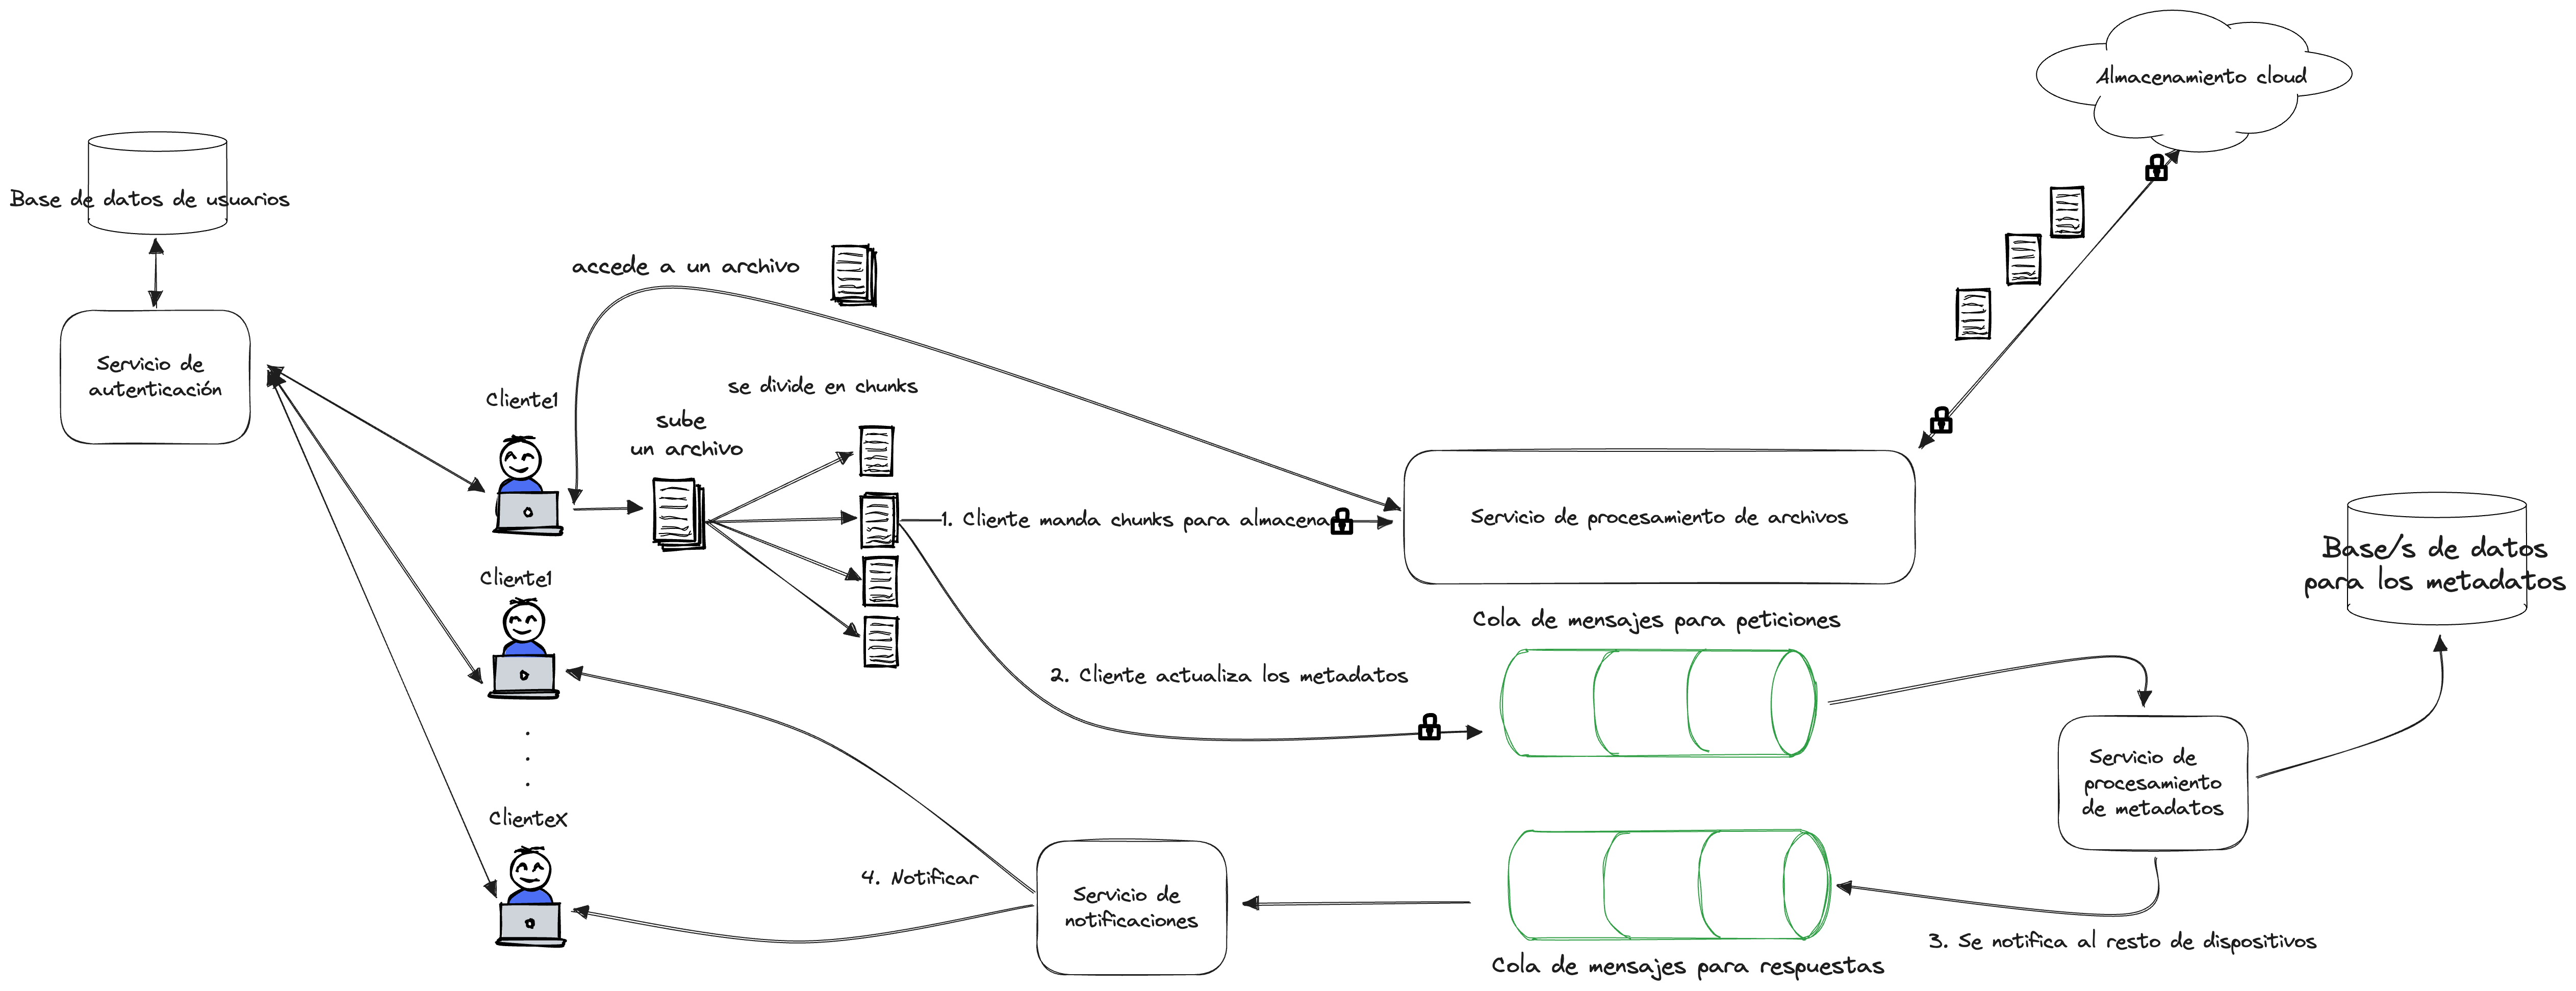
\includegraphics[width=\textwidth]{images/diagramacentral.png}
  \caption{Posible arquitectura de un servicio centralizado de archivos}
\end{sidewaysfigure}


\subsubsection{Arquitectura de IPFShare: un sistema de intercambio de archivos descentralizado}

\section{Tecnologías}
\subsection{Tecnologías propuestas}
\subsection{Tecnologías usadas}


\section{Implementación}


\begin{minted}{typescript}
import OrbitDB from "orbit-db"
// eslint-disable-next-line @typescript-eslint/ban-ts-comment
// @ts-ignore
import AccessController from "orbit-db-access-controllers/interface"
import DocumentStore from "orbit-db-docstore"
import { IdentityProvider } from "orbit-db-identity-provider"

export interface RegistryEntry {
    peerId: string
    orbitdbIdentity: string // DID
    username: string // alias
  }

export abstract class Registry<S, DocType> {
    abstract accessController: AccessController
    abstract store: S
    abstract open(): Promise<void>
    abstract create(): Promise<void>
    abstract replicate(): Promise<void>
    abstract close(): Promise<void>
    abstract addUser(user: DocType): Promise<void>
    abstract getUser(entryId: string): Promise<DocType | undefined>
    abstract updateUser(entryId: string, updates: Partial<DocType>): Promise<void>
    abstract searchUsers(queryFn: (entry: DocType) => boolean): Promise<DocType[]>
    abstract deleteUser(entryId: string): Promise<void>
  }
\end{minted}